% 04-results — v1.0
% Sayilar results/summary.json (N=109), paired.json, alpha_site_sensitivity.json (N=109),
% icc.json (N=10), csp.json (N=10), affective.json (N=18) dosyalarindan alindi.

\subsection*{Channel reduction, bandwidth and quantisation do not degrade alpha reactivity}
At the full montage the eyes-closed/eyes-open alpha log ratio was $0.91$
(95\% CI $[0.78, 1.04]$; $N=109$). The Fz single-channel chain --- single electrode,
128\,Hz, 1\,\textmu V quantisation, 1--40\,Hz band-limiting --- gave $0.77$
($[0.65, 0.89]$). Comparing the single channel with the scalp average, the paired
difference was $-0.14$ ($[-0.19, -0.09]$). The mean per-subject retention ratio was
$0.90$ ($[0.85, 0.96]$) and the geometric estimator (ratio of means) was $0.87$; the
two estimators differ because ratios are skewed and both are reported in
\texttt{results/paired.json} and \texttt{inference.json}.

That comparison is confounded by electrode site. Two corrections are needed. First, the
acquisition chain itself costs almost nothing to \emph{reactivity}: keeping the same
electrode (Fz in the full recording versus Fz after the chain), the paired difference was
$-0.0001$ ($[-0.0004, 0.0001]$), i.e.\ \textbf{99.99\%} of the reactivity effect was
retained; the corresponding retention interval $[0.9996, 1.0001]$ is stored in
\texttt{results/site\_metrics.json} (\texttt{chain\_retention}). Second, the electrode-site decision is not free: eyes-closed alpha power at Fz
is only about \textbf{58\%} of the posterior-channel average (ratio $0.58$,
$[0.52, 0.63]$). A single-channel device therefore pays for its site choice, not for its
sampling or bandwidth. This also explains why 128\,Hz sampling, 1\,\textmu V quantisation and a 40\,Hz
low-pass left the estimate essentially unchanged: the band versus quantisation contrast
was $-0.00012$ (retention $0.9999$, $p=0.007$), which is negligible for 8--12\,Hz Welch
power and consistent with earlier filter work \cite{tanner2015filters}.

Table~\ref{tab:alpha} reports the condition means and Figure~\ref{fig:pipeline}
shows the degradation grid, while Figure~\ref{fig:retention} shows retention.

\begin{table}[H]
  \centering
  \caption{Alpha reactivity by condition ($N=109$; mean log ratio with 95\% CI). Noise
  and blink arms are separate; the final row combines both.}
  \label{tab:alpha}
  \begin{tabular}{lcc}
    \hline
    Condition & Log ratio & 95\% CI \\
    \hline
    Full montage (64 ch average) & 0.91 & [0.78, 1.04] \\
    Single channel (Fz) chain & 0.77 & [0.65, 0.89] \\
    + noise 20\,dB & 0.76 & [0.64, 0.88] \\
    + noise 10\,dB & 0.70 & [0.58, 0.83] \\
    + noise 5\,dB & 0.60 & [0.48, 0.72] \\
    + noise 0\,dB & 0.38 & [0.26, 0.50] \\
    + blinks 5/min & 0.77 & [0.65, 0.89] \\
    + blinks 15/min & 0.77 & [0.65, 0.89] \\
    + blinks 30/min & 0.77 & [0.65, 0.89] \\
    + noise 0\,dB and blinks 30/min & 0.39 & [0.27, 0.51] \\
    \hline
  \end{tabular}
\end{table}


\begin{figure}[H]
  \centering
  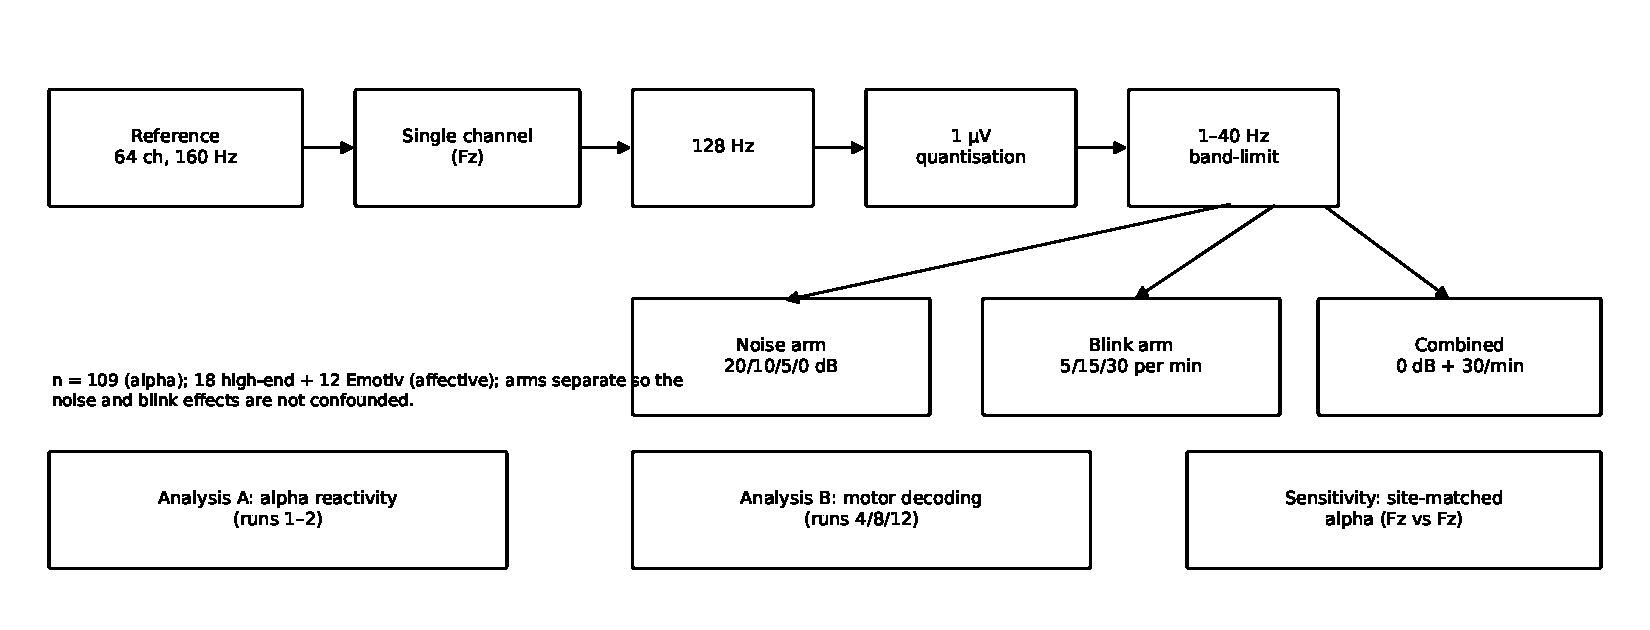
\includegraphics[width=\linewidth]{figures/fig1_pipeline.pdf}
  \caption{Degradation tree. The reference is the full-montage recording; the
  single-channel chain is cumulative, while the noise and blink arms branch from the
  fully degraded chain and are analysed separately.}
  \label{fig:pipeline}
\end{figure}

\subsection*{Noise is the constraint that matters; blinks alone do not shift alpha reactivity}
Noise produced a monotonic dose-response: $0.76$ at 20\,dB, $0.71$ at 10\,dB, $0.60$
at 5\,dB and $0.38$ at 0\,dB. Relative to the clean single-channel chain (the correct
baseline for an incremental contamination), the geometric retention was $0.99$, $0.94$,
$0.85$ and $0.68$; relative to the full-montage reference it was $0.86$, $0.82$, $0.73$
and $0.59$. The incremental paired contrasts
against the clean chain (which isolate the noise manipulation) were $-0.008$
($[-0.011, -0.006]$) at 20\,dB, $-0.064$ ($[-0.075, -0.052]$) at 10\,dB, $-0.169$
($[-0.197, -0.140]$) at 5\,dB and $-0.384$ ($[-0.441, -0.328]$) at 0\,dB; all survive
Benjamini--Hochberg correction across the condition family ($q<0.001$). The three blink arms were almost identical to
the clean chain ($0.77$ at 5 and 15/min, $0.77$ at 30/min). The incremental contrast (30 blinks/min minus
clean chain) was $-0.002$ ($[-0.003, -0.001]$; $q=0.0005$), a change of about 0.2\% that
is statistically detectable but negligible in size; the combined arm ($0.39$) was driven
by the 0\,dB noise it contains. The injected template has almost no energy in 8--12\,Hz
and the same rate was added to both conditions, so this null is close to guaranteed by
construction and should be read as a model check, not as evidence about real blinks;
ocular artifacts are known to bias broadband power in ways this additive model does not
represent \cite{hagemann2001ocular}.
The template has almost no 8--12\,Hz energy and the same rate is added to both
conditions, so the null is close to guaranteed and is not evidence about real ocular
contamination \cite{gratton1983ocular,croft2000ocular,whitham2007emg}.

\begin{figure}[H]
  \centering
  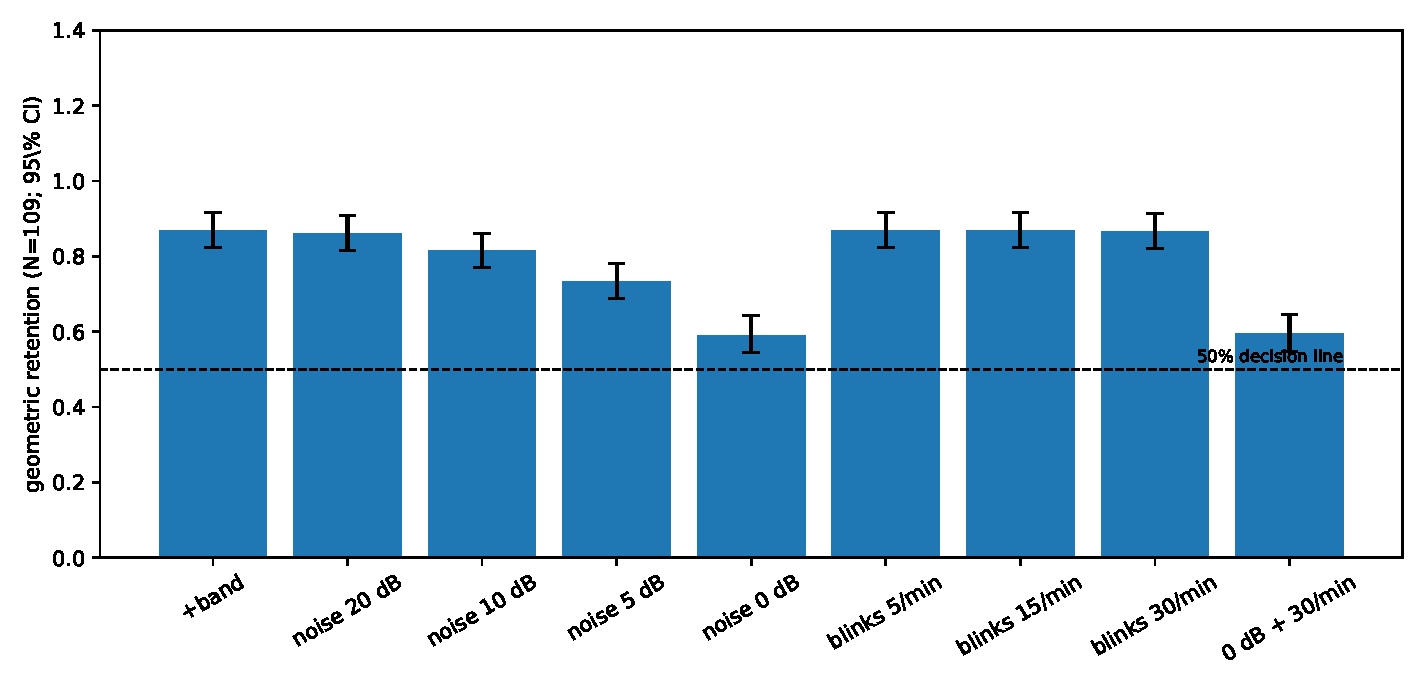
\includegraphics[width=0.85\linewidth]{figures/fig2_retention.pdf}
  \caption{Alpha reactivity retained relative to the clean single-channel chain, by
  condition ($N=109$; geometric retention and 95\% CI). The dashed line is the planned
  50\% decision threshold. Noise reduces retention monotonically; the blink arm is a
  model check and is not a real-blink test.}
  \label{fig:retention}
\end{figure}

\subsection*{Affective decoding survives a full montage but not one electrode}
Table~\ref{tab:affective} reports the affective arm on the high-end BrainVision
recordings (18 recordings from 20 participants; about 10 trials per quadrant). From the
full montage, valence was decoded at $0.69$ ($[0.62, 0.76]$), arousal at $0.68$
($[0.60, 0.75]$) and the four quadrants at $0.58$ ($[0.49, 0.67]$); the binary
intervals exclude chance and the four-class interval is above it. From the same data
reduced to the single-channel chain, valence showed no significant evidence of above-chance decoding ($0.52$; $[0.47, 0.57]$, $p=0.45$)
--- arousal to $0.56$ ($[0.50, 0.62]$), which remains above chance but far below the
montage, and the four quadrants to $0.34$ ($[0.27, 0.41]$). The paired full-minus-single
differences were $+0.17$ ($[0.10, 0.24]$) for valence, $+0.12$ ($[0.03, 0.20]$) for
arousal and $+0.24$ ($[0.14, 0.34]$) for the four quadrants, so the collapse is not
just a loss of significance.

A low-cost 14-channel Emotiv headset decoded the same targets at $0.67$
($[0.57, 0.77]$) for valence, $0.71$ ($[0.63, 0.79]$) for arousal and $0.56$
($[0.46, 0.67]$) for the four quadrants. On the 12 participants present in both
datasets, the low-cost minus high-end difference was $-0.07$ ($[-0.21, 0.08]$) for
valence, $+0.05$ ($[-0.05, 0.15]$) for arousal and $-0.04$ ($[-0.21, 0.12]$) for the
four quadrants. These differences are not statistically distinguishable from zero, but
a $\pm 10$-point equivalence test does not pass either (TOST $p=0.31$, $0.14$ and
$0.23$), so we describe the low-cost device as performing at a similar
level in this sample, not that equivalence has been established.

\begin{table}[H]
  \centering
  \caption{Affective decoding by acquisition representation: high-end full montage
  ($N=18$ recordings), low-cost 14-channel Emotiv ($N=12$), and high-end data
  reduced to one degraded channel ($N=18$). Balanced accuracy with 95\% CI;
  chance 0.50 (binary) and 0.25 (four-class).}
  \label{tab:affective}
  \begin{tabular}{lccc}
    \hline
    Target & High-end montage & Low-cost 14 ch & Single channel \\
    \hline
    Valence & 0.69 [0.62, 0.76] & 0.67 [0.57, 0.77] & 0.52 [0.47, 0.57] \\
    Arousal & 0.68 [0.60, 0.75] & 0.71 [0.63, 0.79] & 0.56 [0.50, 0.62] \\
    Four quadrants & 0.58 [0.49, 0.67] & 0.56 [0.46, 0.67] & 0.34 [0.27, 0.41] \\
    \hline
  \end{tabular}
\end{table}


\begin{figure}[H]
  \centering
  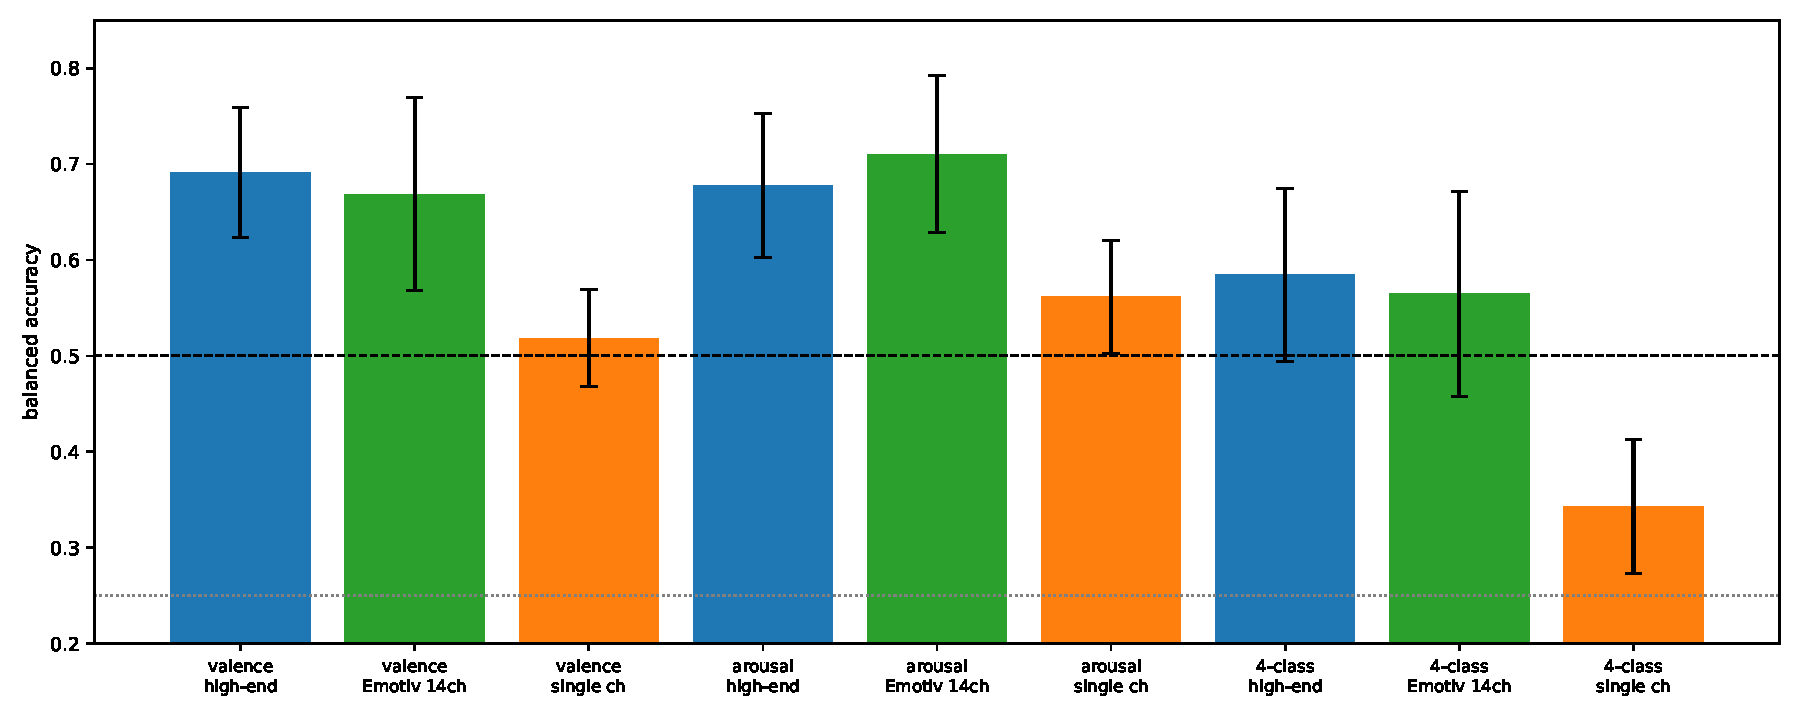
\includegraphics[width=0.9\linewidth]{figures/fig3_affective.pdf}
  \caption{Affective decoding by acquisition representation: high-end montage,
  low-cost 14-channel Emotiv and single-channel chain. Dashed and dotted lines mark
  chance for binary (0.50) and four-class (0.25) targets.}
  \label{fig:affective}
\end{figure}

\subsection*{Decomposing the affective collapse: representation, site and band}
The chain that is harmless for alpha is also harmless for affective decoding
(Table~\ref{tab:decomp}): resampling to 128\,Hz, quantisation and band-limiting left
four-class accuracy at $0.58$--$0.59$ and valence at $0.69$--$0.70$. The loss appears
when the representation becomes one electrode. Valence was not distinguishable from
chance at any of the four sites ($0.51$--$0.53$ at Fz, Cz, Pz and Oz); four-class
accuracy was $0.33$--$0.38$, above the $0.25$ chance level but far below the montage;
and arousal was weakly above chance at Fz, Pz and Oz before correction ($0.56$--$0.57$;
unadjusted $p\approx0.04$) but not at Cz ($0.56$, $[0.49, 0.62]$). The single-Fz arousal
value survives the six-contrast affective family ($q=0.0496$) but not the 12-test site
sweep ($q\approx0.079$); we therefore treat the site-level arousal pattern as
exploratory. With only four midline sites and three features per site, the
bounded claim is that none of these single-electrode representations approached the
montage, not that every possible electrode would fail.

A band control changes the interpretation of the full-montage result. With only theta
and alpha features the full montage decoded valence at $0.60$ ($[0.54, 0.66]$) and the
four quadrants at $0.46$ ($[0.38, 0.53]$), whereas beta-only features retained $0.70$
($[0.61, 0.79]$) and $0.62$ ($[0.53, 0.71]$). A substantial part of the
full-montage affective advantage therefore sits in the beta band, where EMG
contamination is a known concern \cite{whitham2007emg,goncharova2003emg}. Because
beta-only decoding was at least as high as the full montage ($0.70$ vs $0.69$ for
valence, $0.62$ vs $0.58$ for four-class), we do not interpret the montage advantage as
purely additive cortical information, and we did not measure EMG directly. This is an
interpretation, not a tested mechanism.

\begin{table}[H]
  \centering
  \caption{Decomposition of affective decoding (18 high-end recordings; balanced
  accuracy). Chance is 0.50 for valence/arousal and 0.25 for four-class.}
  \label{tab:decomp}
  \begin{tabular}{lccc}
    \hline
    Representation & Valence & Arousal & Four-class \\
    \hline
    Full montage, all bands & 0.69 & 0.68 & 0.58 \\
    Full montage, theta+alpha only & 0.60 & 0.63 & 0.46 \\
    Full montage, beta only & 0.70 & 0.70 & 0.62 \\
    128\,Hz / quantised / band-limited & 0.70 & 0.68 & 0.58 \\
    Single Fz & 0.52 & 0.56 & 0.34 \\
    Single Cz & 0.51 & 0.56 & 0.38 \\
    Single Pz & 0.52 & 0.56 & 0.33 \\
    Single Oz & 0.53 & 0.57 & 0.35 \\
    \hline
  \end{tabular}
\end{table}


\begin{figure}[H]
  \centering
  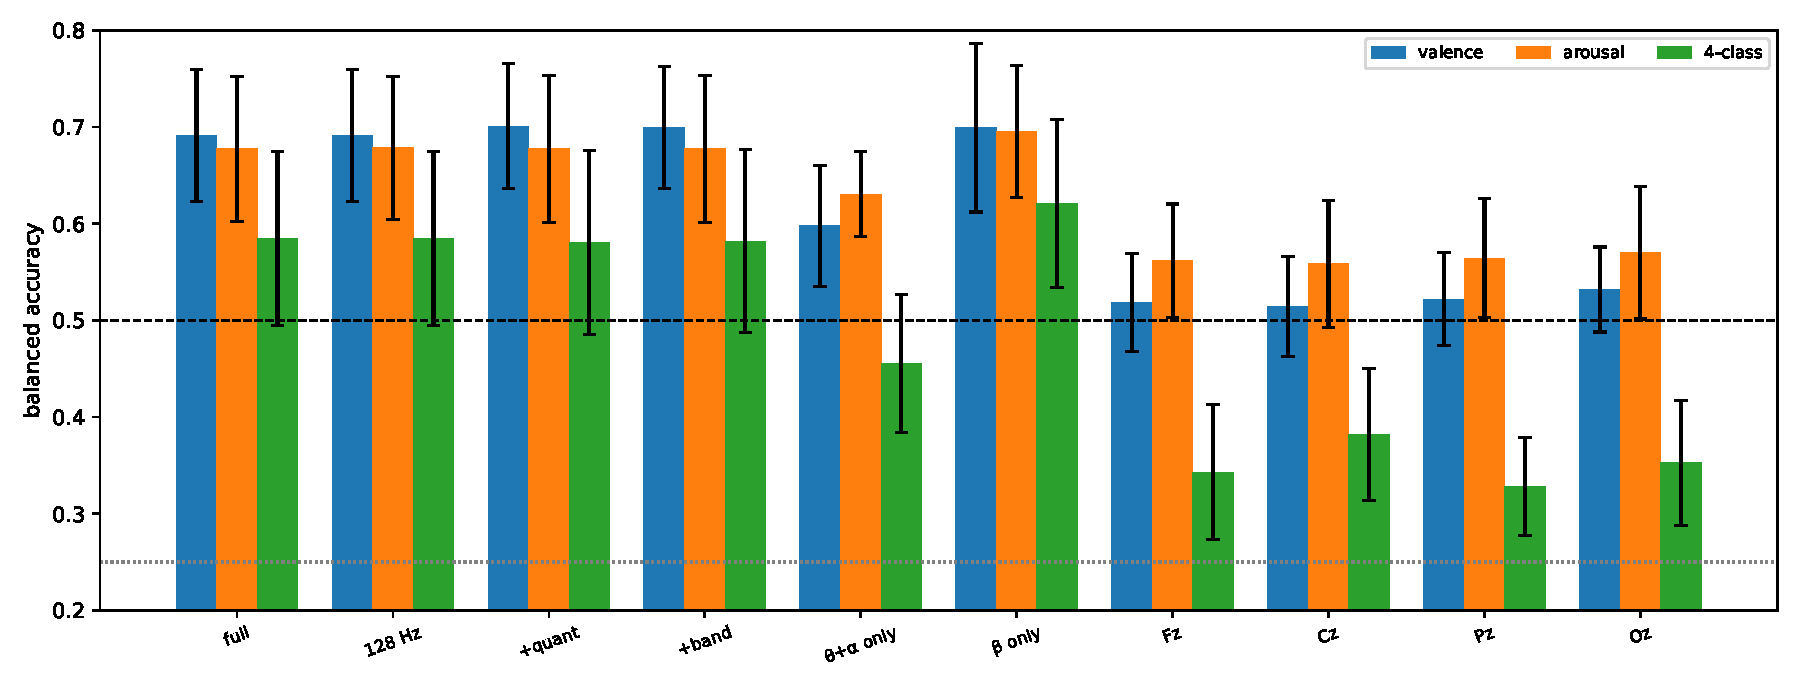
\includegraphics[width=\linewidth]{figures/fig4_decomp.pdf}
  \caption{Decomposition of affective decoding by acquisition step and band. The
  dashed and dotted lines mark chance for binary (0.50) and four-class (0.25) targets.}
  \label{fig:decomp}
\end{figure}

\subsection*{Reliability depends on the timescale}
Short-lag stability of consecutive 2\,s alpha windows was $r_{SB}=0.016$
($[-0.08, 0.11]$; $N=109$). This is a short-lag stability measure, not a classical
reliability coefficient: odd and even 2\,s windows are separated by about two
seconds. It says
that a momentary alpha estimate is noisy and is consistent with zero. In the ten-subject
subset with three repeated imagined-hand runs, block-level alpha power had
ICC(2,1)$=0.92$, which captures stable between-subject differences. The two are not
contradictory, and neither is a test--retest coefficient across sessions; published
single-channel test--retest work reports ICCs of roughly 0.76--0.85 for eyes-closed
relative power \cite{rogers2016reliability}, but on a different design.

\subsection*{Exploratory motor decoding was inconclusive}
In the ten-subject subset with imagery runs, balanced accuracy for imagined
left/right hand was $0.51$ ($[0.47, 0.56]$) at Fz and $0.54$ ($[0.46, 0.62]$) at the
full montage; a CSP reference reached $0.52$ ($[0.41, 0.63]$) and a sensorimotor subset
$0.55$ ($[0.44, 0.66]$). Every interval includes chance, and the full-montage decoder
has more features than trials (64 channels, 45 trials). Figure~\ref{fig:decoding} shows the distribution of these accuracies.
Because the reference decoder itself did not exceed chance, this arm cannot test the
decoding hypothesis; it is reported as \textbf{invalid}, not merely inconclusive, and
is not used for any claim.

\begin{figure}[H]
  \centering
  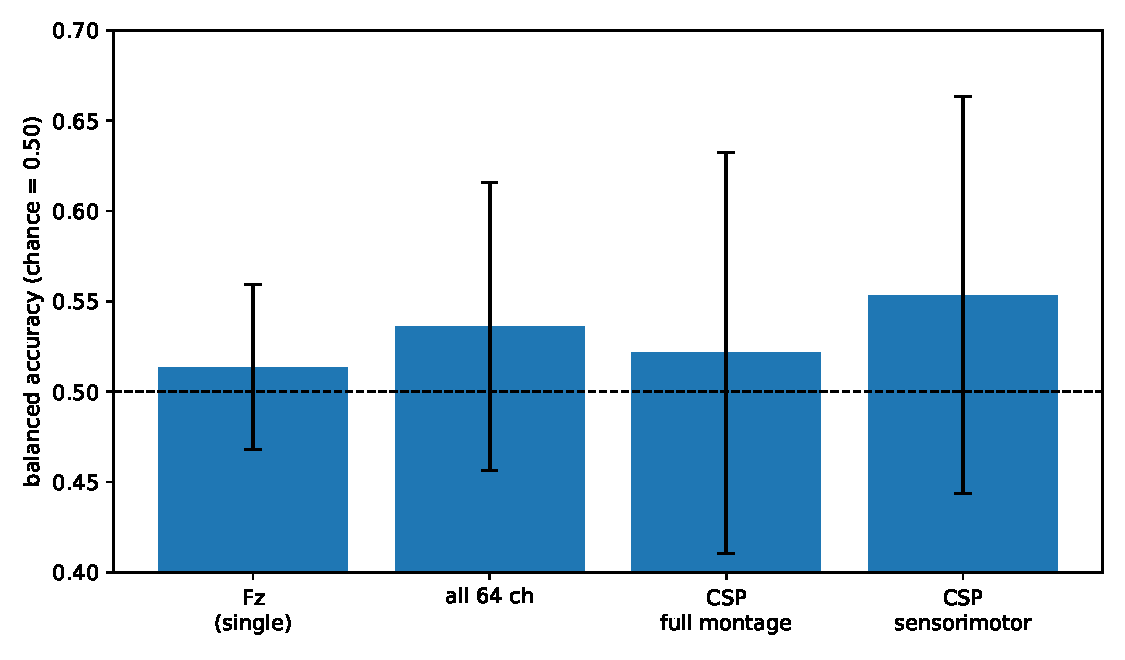
\includegraphics[width=0.9\linewidth]{figures/fig5_decoding.pdf}
  \caption{Exploratory motor-imagery decoding ($N=10$), balanced accuracy by
  representation. All intervals include chance (0.50).}
  \label{fig:decoding}
\end{figure}

\subsection*{Decision matrix}
Table~\ref{tab:decision} applies the planned 50\% retention rule to the outcomes
that were estimated.

\begin{table}[H]
  \centering
  \caption{Claim-level verdicts.}
  \label{tab:decision}
  \begin{tabular}{p{0.40\linewidth}p{0.28\linewidth}p{0.24\linewidth}}
    \hline
    Claim & Evidence & Verdict \\
    \hline
    Alpha reactivity survives the acquisition chain & Same-site reactivity retention lower bound 0.9996 & Supported \\
    Alpha reactivity survives 20--5\,dB noise & Clean-chain retention lower bounds 0.99, 0.93, 0.82 & Supported \\
    Alpha reactivity survives 0\,dB noise & Clean-chain retention 0.68 [0.64, 0.72] & Supported (attenuated) \\
    Combined 0\,dB + 30 blinks/min & Clean-chain retention 0.68 [0.65, 0.71] & Supported (attenuated) \\
    Blinks bias alpha reactivity & Clean-chain retention 0.998 in a spectrally orthogonal, symmetric model & Not a real-blink test (H1 untested) \\
    Pre-specified 60\% balanced-accuracy floor & Valence full passes (lower 0.62); four-class full fails (lower 0.49); Emotiv valence fails (lower 0.57); arousal full/Emotiv pass & Mixed; reported as auxiliary criterion \\
    Single-trial motor decoding above chance & Reference decoder did not exceed 0.50 & Invalid (not testable) \\
    Momentary individual-level alpha reliability & Short-lag stability $r_{SB}=0.016$ & Not supported \\
    Stable individual alpha level & ICC across runs 0.92 (no CI) & Supported (block-level) \\
    \hline
  \end{tabular}
\end{table}

\noindent
\textbf{Status.} The alpha arm uses the full 109-subject dataset. The
affective arm uses 18 high-end recordings and 12 low-cost Emotiv recordings; the Emotiv
alignment relies on wall-clock timestamps and 8 participants are dropped. The
full-montage affective advantage is partly beta-band and may include a muscular
contribution. The motor arm is invalid (reference at chance) and underpowered; H5 is untested. These scope limits are
stated in the Discussion and are not treated as results.
